\chapter{Réalisation}

\section{Introduction}
 
Après avoir planifié le projet, nous allons entamer le troisième chapitre dans lequel nous détaillerons le cycle de développement de l'application de générateur de formulaires.

\section{Choix technologiques  et  environnements de développement}
Le but de cette partie est d’obtenir un sprint qui va nous permettre de gérer l'authentification User et Admin et la première partie de la création d'un formulaire.
\subsection{Implémentation}
Nous arriverons à ce stade à rassembler nos informations et à réaliser notre système.\\
Pour commencer, nous allons tester tout d’abord les services web développés dans la partie Back End afin de garantir
la bonne communication entre le Front et le Back et l’application. Ensuite, nous allons montrer les interfaces de l’application correspondantes à ce sprint.

    \newpage
\subsubsection{Test de l'application }  
La figure \ref{logintest} présente l’interface de connexion où l’utilisateur doit saisir ses coordonnées pour accéder
à l’application.  
\begin{figure} [H]
    \centering
         \begin{center}
             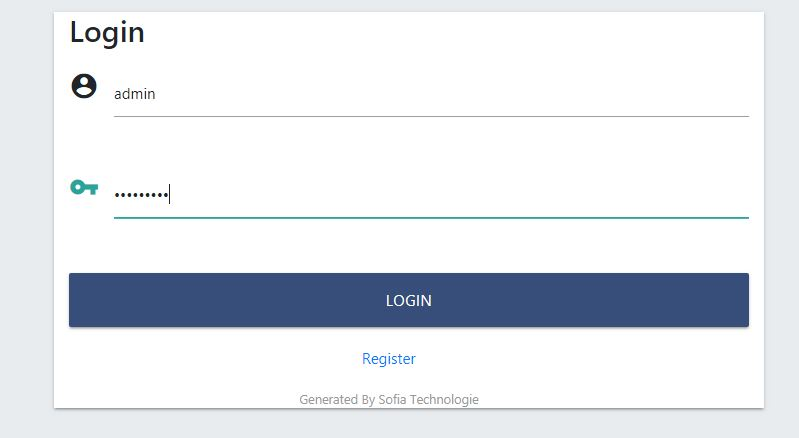
\includegraphics [width=16cm,height=8cm] {SprintImage/interfaceLogin.JPG}
            \caption{Interface Login}
            \label{logintest}
        \end{center}
    \end{figure}   
S’il y a une erreur de saisie dans l’interface login un message d’erreur va être affiché comme illustre la figure \ref{logintest1}.
\begin{figure} [H]
    \centering
         \begin{center}
             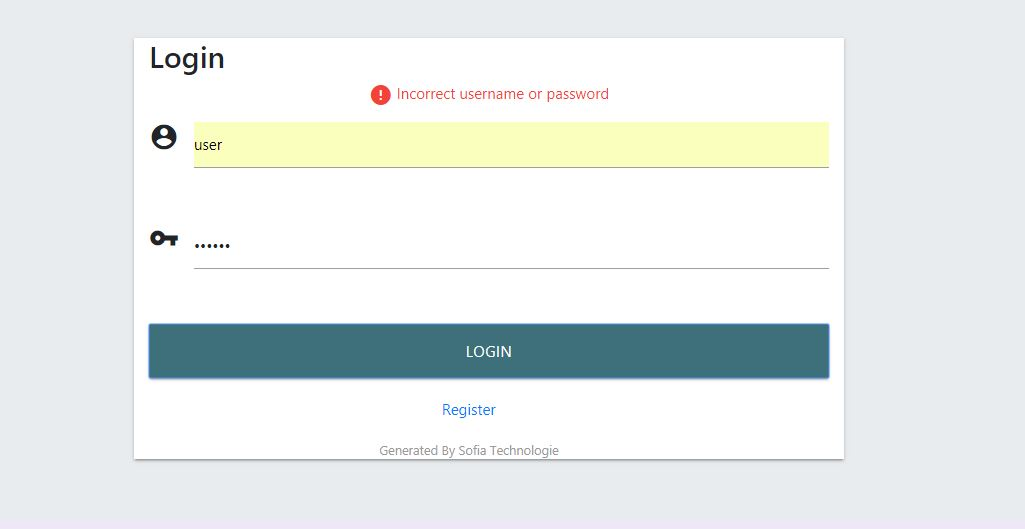
\includegraphics [width=16cm,height=8cm] {SprintImage/loginfailed.JPG}
            \caption{Erreur Login}
            \label{logintest1}
        \end{center}
    \end{figure}
la figure \ref{register} présente le mur de la création d'un compte dans le cas ou un utilisateur ne possède pas un compte.
\begin{figure} [H]
    \centering
         \begin{center}
             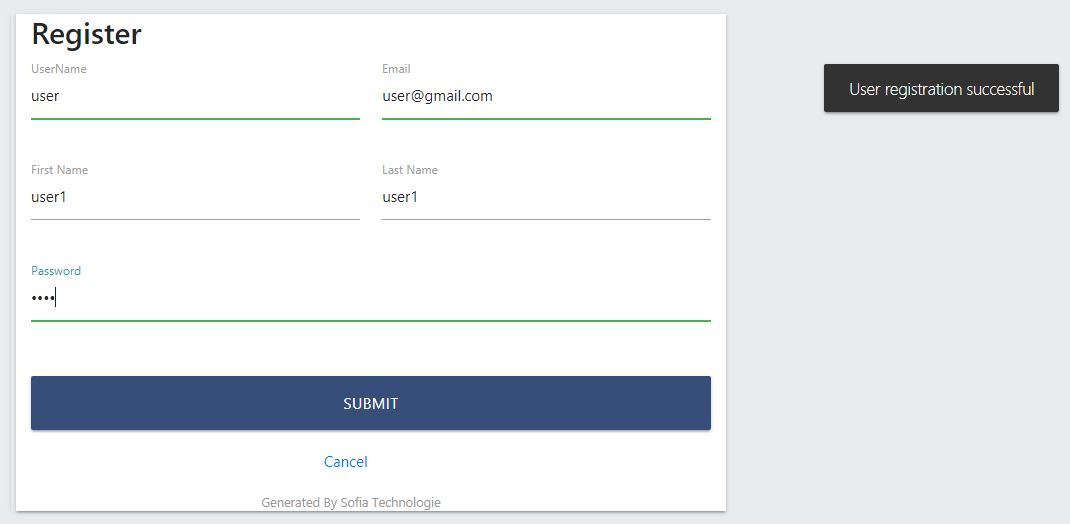
\includegraphics [width=16cm,height=9cm] {SprintImage/register.JPG}
            \caption{Register d'un user}
            \label{register}
        \end{center}
    \end{figure}
Après l'authentification en tant qu'un Admin,la figure \ref{form1} présente l’interface globale de la création d'un formulaire. 
\begin{figure} [H]
    \centering
         \begin{center}
             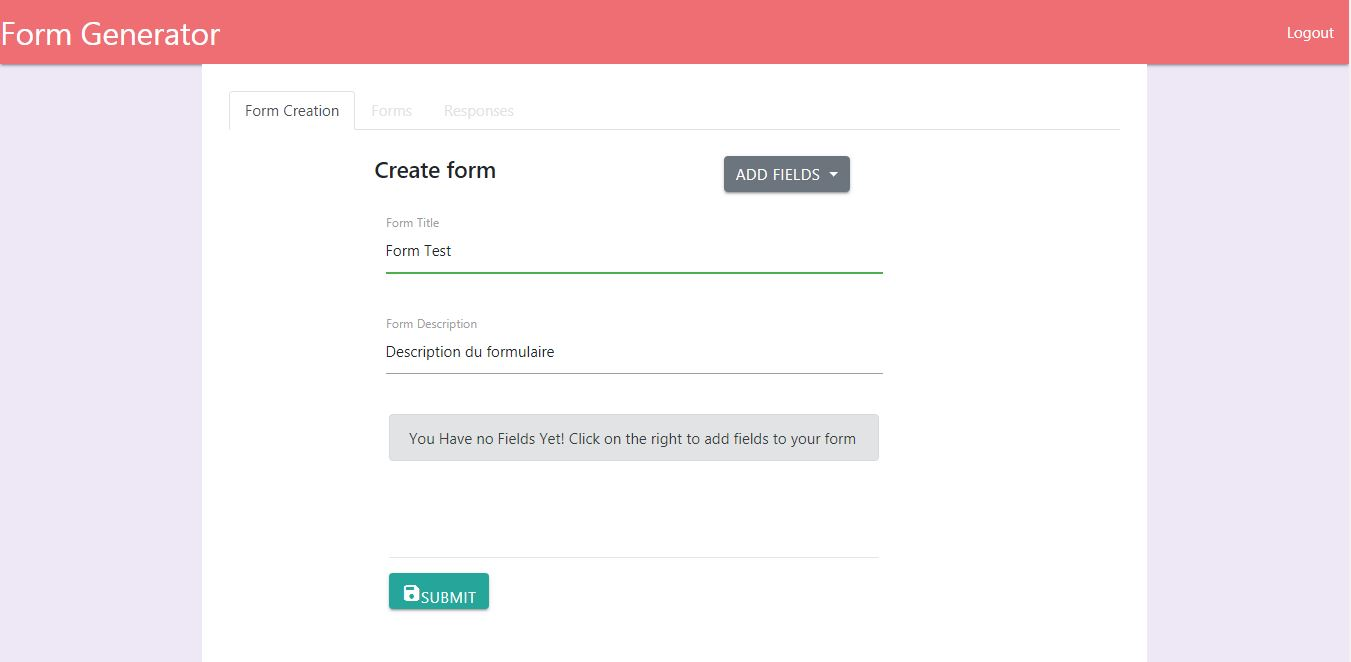
\includegraphics [width=16cm,height=9cm] {SprintImage/Form1.JPG}
            \caption{Interface globale de la création d'un formulaire}
            \label{form1}
        \end{center}
    \end{figure}
%ici la partie du sprint 2 .............................

\section{Sprint2}
Après avoir obtenu le premier incrément de notre application, nous allons passer au deuxième sprint qui englobe les fonctionnalités délicates de notre projet.
Nous allons également répéter les mêmes étapes du premier Sprint.
\newpage

\subsection{Implémentation}
Après avoir illustrer l’enchainement de différentes étapes de la création du formulaire avec le diagramme de séquence ci dessus, nous abordons maintenant l’étape qui se suit.
\subsubsection{Test des services web}
Dans cette étape, nous allons tester les services web développés au cours de ce sprint.

\newpage

\subsubsection{Test de l'application }  
la création d'un formulaire est illustré par la figure \ref{fig1}.
    \begin{figure} [H]
    \centering
         \begin{center}
             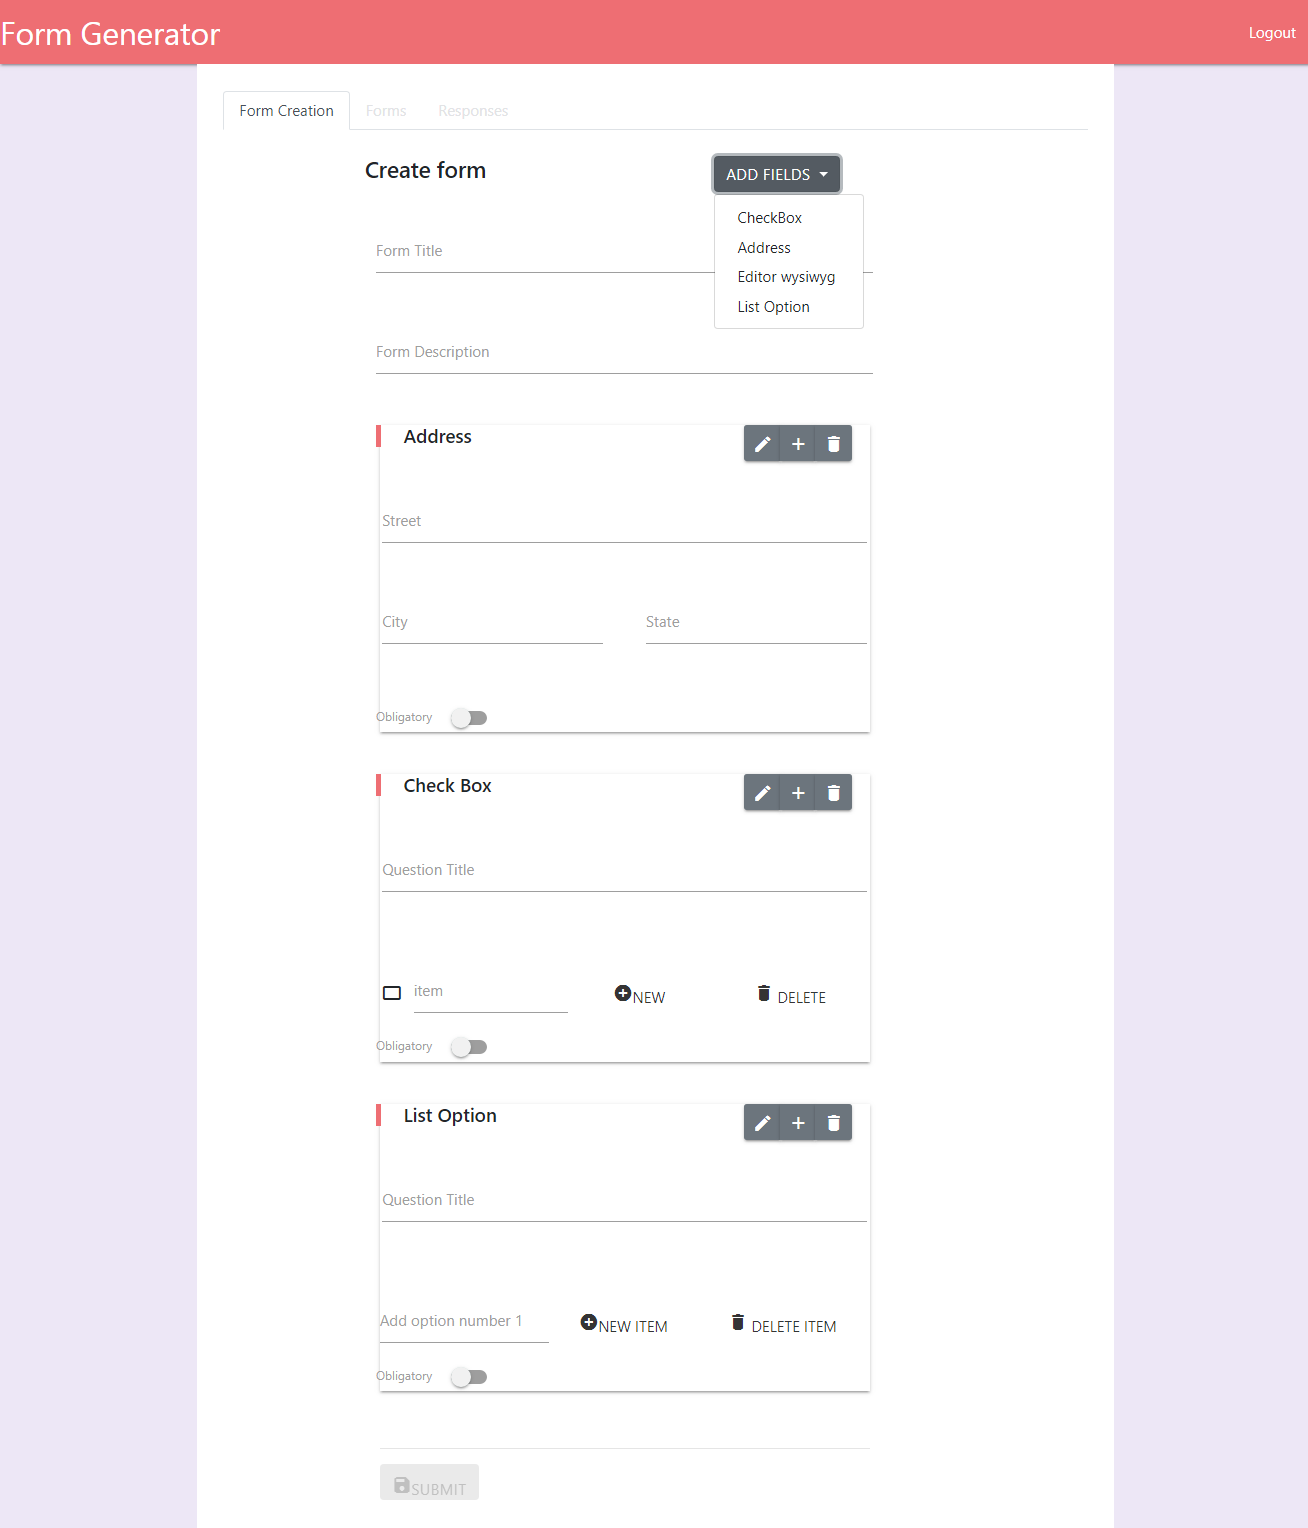
\includegraphics [width=16cm,height=14cm] {SprintImage/Formulaire.png}
            \caption{Mur de la création d'un formulaire}
            \label{fig1}
        \end{center}
    \end{figure}
\newpage  
L'affichage des formulaires disponible avec la possibilité d'entraîner une modification ou la suppression est montré par la figure \ref{fig2} suivante.
   \begin{figure} [H]
    \centering
         \begin{center}
             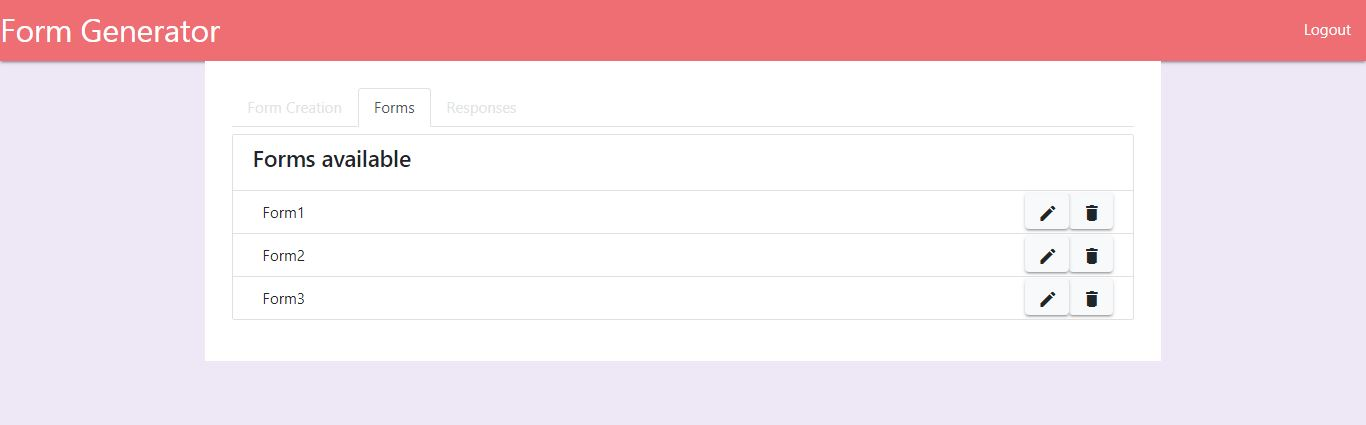
\includegraphics [width=16cm,height=7cm] {SprintImage/FormAvailable.JPG}
            \caption{Mur de la modification/suppression d'un formulaire}
            \label{fig2}
        \end{center}
    \end{figure}
\section{Sprint3}
Pour ce troisième sprint, nous allons se concentrer sur la partie de soumission de la réponse sur des formulaires disponibles. Nous allons traiter la fonctionnalité « Remplissage du formulaire et soumission ».

\subsection{Implémentation}
Une fois l’enchaînement du processus de soumission détaillé, nous abordons maintenant la dernière étape de notre sprint les tests des web services ainsi les différentes interfaces correspondantes.
\subsubsection{Test des services web}
La figure \ref{fig5} illustre le web service qui permet de confirmer la réponse à un formulaire.
\subsubsection{Test de l'application }  
L'interface globale du formulaire dans laquelle l'utilisateur fournit sa réponse est présentée dans la figure  \ref{fig6}.
\begin{figure} [H]
    \centering
         \begin{center}
             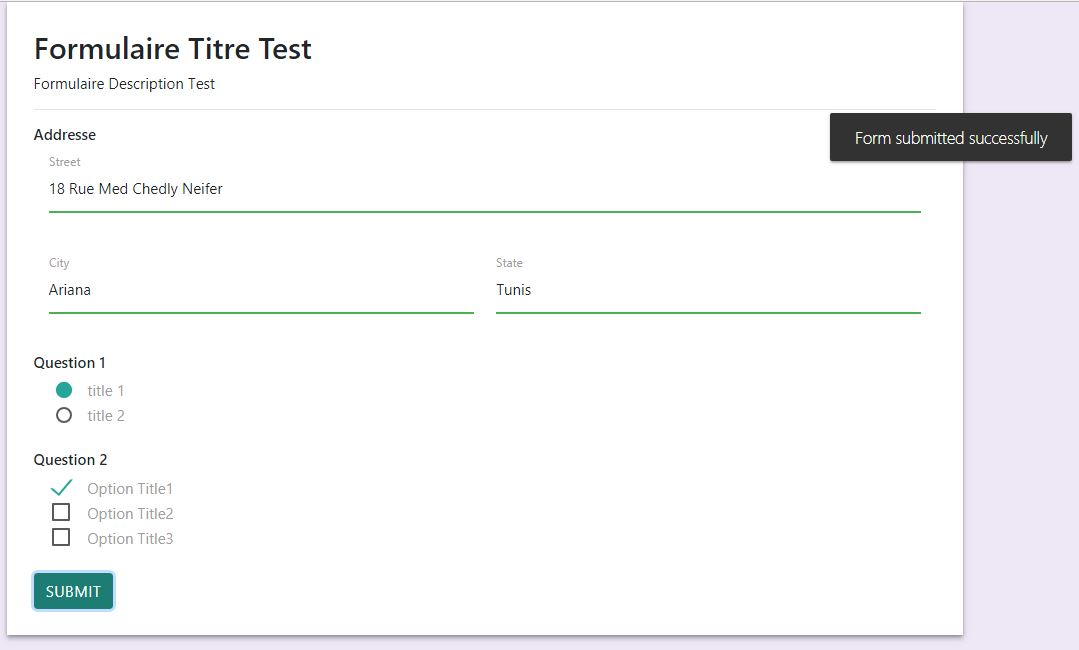
\includegraphics [width=16cm,height=8cm] {SprintImage/interfaceForm.JPG}
            \caption{Soumettre la réponse }
            \label{fig6}
        \end{center}
    \end{figure}
%\section{Sprint4}

\section{Conclusion}
Nous avons réussi à élaborer les différents phases d’analyse en détaillant la réalisation des sprints qui nous permettent d'avoir comme finalité notre système. \\
Le chapitre suivant sera consacré pour détailler les ressources
que nous avons utilisées pour accomplir notre projet.